\documentclass{letter}

\usepackage{csquotes}
\usepackage[margin=1in]{geometry}
\usepackage{tikz}
\usepackage{amsmath}
\usepackage{enumitem}

\newcommand{\heading}[1]{{\large \textsc{#1}}}

\begin{document}

\heading{COMP 282 - Final (Fall, 2018)}
\kern 2cm
\heading{Name:}

{\bf Question 1} \kern 1cm Give the best data structure to use in the following
scenarios.  Justify your answer.  You may assume sufficient system resources to
support whichever data structure you choose. 


\begin{enumerate}[label=(\alph*)]

\item You want to store a large number of integers.  They do not change often,
but you need to be able to search them quickly.

\vspace{3cm}

\item You need to be able to store an unknown number of floating point values.
You only need to access and delete latest value that had been stored.

\vspace{3cm}

\item You want to store a large number of integers.  They change often, and you
need to search them quickly.

\vspace{3cm}

\item You have a series of bank records, consisting of a name, account number,
and balance.  You need to be able to quickly insert new records, update a given
record, and delete records.

\vspace{3cm}

\item You have a very small number of strings.  You do not need to insert or
delete strings, but you do need to search them quickly.

\end{enumerate}

\clearpage

{\bf Question 2} \kern 1cm Use {\em Djikstra's algorithm} to find all-pairs
shortest paths from $v_0$ to vertices in its connected component in the
following graph.

\begin{equation*}
V = \{ v_0, v_1, v_2, v_3, v_4, v_5, v_6, v_7 \}
\end{equation*}

\begin{tabular}{ c | c }
Edge & Weight \\ \hline
$\{ v_0, v_1 \}$ & 4 \\
$\{ v_0, v_3 \}$ & 6 \\
$\{ v_0, v_6 \}$ & 3 \\
$\{ v_1, v_4 \}$ & 2 \\
$\{ v_1, v_2 \}$ & 2 \\
$\{ v_2, v_3 \}$ & 1 \\
$\{ v_2, v_7 \}$ & 4 \\
$\{ v_3, v_4 \}$ & 2 \\
$\{ v_3, v_5 \}$ & 1 \\
$\{ v_3, v_7 \}$ & 7 \\
$\{ v_4, v_5 \}$ & 6 \\
$\{ v_4, v_6 \}$ & 1 \\
$\{ v_6, v_7 \}$ & 4 \\
$\{ v_7, v_5 \}$ & 2 \\
\end{tabular}

\clearpage

{\bf Question 3} \kern 1cm Given the following tables, and SQL statement,
construct a table that represents the results you would expect when running
this query.

\begin{center}
\begin{tabular}{ l l }
{\bf Customers} \kern 1cm &
\begin{tabular}{ c | c }
{\bf CustomerId} & {\bf Name} \\ \hline
1 & Bob Roberts \\
2 & Claire McClaireskill \\
3 & Dean VonDeanerson \\
4 & Elanor Elanorsky \\
\end{tabular} \\

\\
\\

{\bf Products} &
\begin{tabular}{ c | c | c }
{\bf ProductId} & {\bf Name} & {\bf Price} \\ \hline
1 & Party Hat & 2.25 \\
2 & Cat-Sized Party Hat & 1.00 \\
3 & Fire-Retardant Sparklers & 4.00 \\
4 & Tactical Pumpkin & 4.50 \\
5 & Turkey-Flavored Cranberry Sauce & 5.00 \\
6 & Chimney Security Alarm & 15.00 \\
\end{tabular} \\

\\
\\

{\bf Orders} &
\begin{tabular}{ c | c | c | c }
{\bf CustomerId} & {\bf ProductId} & {\bf Quantity} & {\bf Date} \\ \hline
2 & 1 & 1 & 2018-01-01 \\
2 & 2 & 3 & 2018-01-01 \\
1 & 4 & 15 & 2018-10-31 \\
4 & 5 & 37 & 2018-11-22 \\
3 & 6 & 1 & 2018-12-25 \\
\end{tabular} \\
\end{tabular}
\end{center}

\begin{verbatim}
SELECT
  c.Name as Name,
  p.Name as Product,
  o.Quantity as Quantity,
  o.Quantity * p.Price as Total
FROM Customers as c, Products as p, Orders as o
WHERE c.CustomerId = o.CustomerId
  AND p.ProductId = o.ProductId
  AND o.Quantity > 3;
\end{verbatim}

\clearpage

{\bf Question 4} \kern 1cm Construct an {\em AVL Tree} by inserting the
following values in order.  Show all intermediate trees, as well as the balance
factor calculated for each node.

\begin{verbatim}
1, 2, 3, 7, 8, 5
\end{verbatim}

\clearpage

{\bf Question 5} \kern 1cm Build a {\em Hash Table} of size 8 by inserting the
following values in order.  Use the algorithm provided to calculate hash
values, and open addressing to resolve all collisions.  Show all intermediate
tables, include both the value and its index in your illustrations.

\begin{verbatim}
12, 456, 137, 10907, 1144, 953, 4, 3713
\end{verbatim}

\begin{verbatim}
int hash (int input) {
  int h = input % 10;
  h += (input / 10) % 10;
  return h % 8;
}
\end{verbatim}

\clearpage

{\bf Question 6} \kern 1cm Briefly explain the following data structures:

\begin{enumerate}[label=(\alph*)]

\item Binary Tree

\vspace{3cm}

\item 2-3-4 Tree

\vspace{3cm}

\item Linked List

\vspace{3cm}

\item Hash Table

\vspace{3cm}

\item Sorted Array

\end{enumerate}

\clearpage

{\bf Question 7} \kern 1cm Give a definition for the following terms:

\begin{enumerate}[label=(\alph*)]

\item Collision Chaining

\vspace{3cm}

\item Adjacent Nodes

\vspace{3cm}

\item Perfect Hashing

\vspace{3cm}

\item Maximum Path Height

\vspace{3cm}

\item Primary Key

\end{enumerate}

\clearpage

{\bf Question 8} \kern 1cm Construct a {\em Red-Black Tree} by inserting the
following values in-order.  Show all intermediate steps.  Indicate a red node
with a dashed circle, and a black node with a solid circle.

\begin{verbatim}
10, 5, 15, 0, 2, 12, 20, 13, 11, 14
\end{verbatim}

\clearpage

{\bf Question 9} \kern 1cm Use Kruskal's algorithm to construct a minimum
spanning forest for the following graph.  Yes, you may the draw graphs.  Show
all steps.

\begin{center}
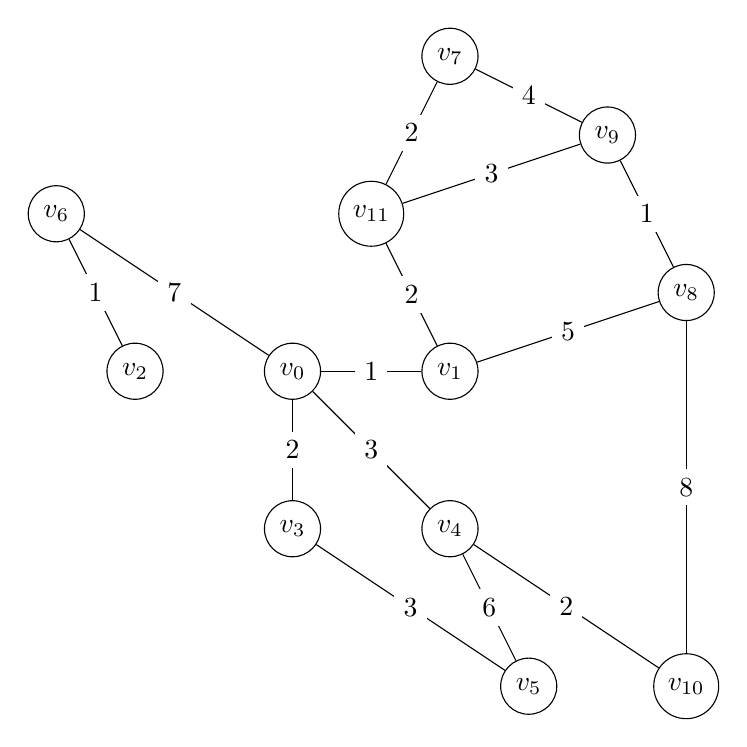
\begin{tikzpicture}
\begin{scope}[every node/.style={circle,draw}]
\node (v0) at (0,0) {$v_0$};
\node (v1) at (2,0) {$v_1$};
\node (v2) at (-2,0) {$v_2$};
\node (v3) at (0,-2) {$v_3$};
\node (v4) at (2,-2) {$v_4$};
\node (v5) at (3,-4) {$v_5$};
\node (v6) at (-3,2) {$v_6$};
\node (v7) at (2,4) {$v_7$};
\node (v8) at (5,1) {$v_8$};
\node (v9) at (4,3) {$v_9$};
\node (v10) at (5,-4) {$v_{10}$};
\node (v11) at (1,2) {$v_{11}$};
\end{scope}

\begin{scope}[every node/.style={fill=white}]
\path (v0) edge node {1} (v1);
\path (v0) edge node {2} (v3);
\path (v0) edge node {3} (v4);
\path (v0) edge node {7} (v6);
\path (v1) edge node {5} (v8);
\path (v1) edge node {2} (v11);
\path (v2) edge node {1} (v6);
\path (v3) edge node {3} (v5);
\path (v4) edge node {6} (v5);
\path (v4) edge node {2} (v10);
\path (v7) edge node {4} (v9);
\path (v7) edge node {2} (v11);
\path (v8) edge node {1} (v9);
\path (v8) edge node {8} (v10);
\path (v9) edge node {3} (v11);
\end{scope}
\end{tikzpicture}
\end{center}

\clearpage

{\bf Question 10} \kern 1cm Is the following function a ``good'' candidate for
a hashing function?  Why or why not?  Supply evidence for your claim.

\begin{verbatim}
public class Hasher {
  public static int hash (int input, int limit) {
    int odd = input;

    if (odd % 2 == 0) odd += 1;

    input = 0;
    while (odd > 0) {
      input += odd % 10;
      odd /= 10;
    }

    return input % limit;
  }
}
\end{verbatim}

\end{document}
